\documentclass{article}

\usepackage{titlesec}
\usepackage{titling}
\usepackage[margin=1cm]{geometry}
\usepackage{float} 
\usepackage{graphicx}
\graphicspath{ {../img/} }
\usepackage{multirow}
\usepackage{booktabs}
\usepackage{hyperref}
\usepackage{xcolor}

\titleformat{\section}
{\Large\bfseries}
{}
{0em}
{}[\titlerule]

\titleformat{\subsection}
{\Large\bfseries}
{}
{0em}
{}

\titleformat{\subsubsection}[runin]
{\bfseries}
{}
{0em}
{}

\titlespacing{\section}
{0em}{0em}{0.5em}
\titlespacing{\subsection}
{0em}{0em}{0em}
\titlespacing{\subsubsection}
{0em}{0em}{1em}

\setlength\intextsep{1mm}

\renewcommand{\maketitle}{
	\begin{center}
		{\huge\bfseries
		\theauthor}
	\end{center}
}

\hypersetup{
  colorlinks=true,
  urlcolor=black!70!black
}

\begin{document}
\title{R\'esumm\'e}
\author{Carlos Herrera Valerio}



\begin{table}[ht]
\centering
	\begin{tabular}{p{5cm}p{6cm}p{6cm}}
	\multirow{3}{*}{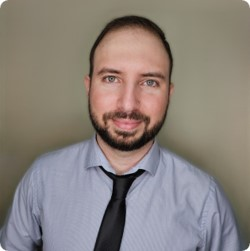
\includegraphics[width=0.16\textwidth]{profile_photo_1-1_rounded}} &
	\multicolumn{2}{c}{\huge\textbf{Carlos Herrera Valerio}} \\
 &
	\begin{tabular}[c]{@{}l@{}}\\Electronic Engineer\\ 8+ years of experience\\ Data Science\\ Analog testing\end{tabular} &
		\multicolumn{1}{r}{\begin{tabular}[c]{@{}r@{}}\\(+506) 8894 4826\\ \href{mailto:carlos.herrera.valerio@gmail.com}{carlos.herrera.valerio@gmail.com}\\ \href{https://www.linkedin.com/in/carlosherreravalerio/}{linkedin.com/in/carlosherreravalerio}\\ Heredia, Costa Rica\end{tabular}} \\
	\multicolumn{1}{l}{} &
 &
\end{tabular}
\end{table}

\section{About me}
\noindent
Electronic Engineer with more than 8 years of experience in the semiconductors industry specialized in high-volume manufacturing, analog testing and electronic design validation. Currently shifting my career towards data science and data analytics applied to manufacturing and problem solving, looking for new work opportunities to align my job to my passion analyzing and understanding data to create a positive impact and bring innovation to the industry.

\section{Work Experience}
\subsection{Intel Costa Rica(2016 - Present day)}
\subsubsection{IO Design Validation of DDR Memory}
\subsubsection{2023 - Present day: }
Work in the Memory IO team, utilizing Lab platform systems to conduct analog validation on DDR interfaces for Intel Xeon projects GNR and SRF. My primary focus was data analysis and standardization, where I automate dataflow using JSL to quickly visualize information and facilitate result reviews. Additionally, I operate measurement equipment—including Scope, BERT, DCPA, VNA, switches, and thermal controllers—via SCPI commands, applying test methodologies within a Python environment.
\subsubsection{IO Design Validation of DDR Memory}
\subsubsection{2022 - 2023: }
For Intel Xeon EMR, I worked remotely as a Product Owner with Santa Clara’s HSIO team. My role involved enabling full test content within an aggressive schedule to prepare for Power On. I frequently had to debug Python scripts and collaborate with designers and Design Validation teams as part of a Task Force to implement the Gen5 Loopback test for UPI interfaces. As a result of the work done during this period, I was awarded for a remarkable, result-oriented effort.
\subsubsection{2019 - 2022: }
Initially working as an individual contributor PDE in the ICX project (Intel Xeon), we were able to achieve PRQ on time, highlighting the work done in data analysis to create an efficient workflow to reduce fallout. Later, I transitioned to the role of Product Owner, where I focused on reducing DPM and improving fallout by implementing multivariable screening based on offline ML results.

\section{Skills}
\noindent\textbf{Data Analysis:} Experience in executing data analysis using JMP and automating tasks with JSL. I’ve also implemented ML models to classify and predict outcomes, calculate associated indicators using Python and R. Additionally, I have worked on distributed computing programming using Docker with PySpark and setup SQL Server ETL processes to deliver dynamic data visualization dashboards using Tableau.\\
\textbf{Linux:} Habituated to work within the Linux environment generating test content, automating and managing files.\\
\textbf{Programming:} Passionate about using data analysis to solve problems. Programming languages/packages: Python, JSL, R, PySpark, Docker, PyTorch, Pandas, SeaBorn, Matplotlib, Sklearn, Postgres, SQL, Tableau.\\
\textbf{Team Work:} With 6 years of experience in High Volume Manufacturing activities, I have actively worked on Task Forces with multidisciplinary engineering teams to properly address silicon issues, debug test content, or reduce high fallout rates. It is common for me to explore volume data in order to select DUTs for specific DOEs.\\
\textbf{Languages:} Excellent written and verbal communication skills in English, and native in Spanish.

\section{Education}

\begin{table}[ht]
\centering
\begin{tabular}{lr}
	\begin{tabular}[c]{@{}l@{}}\textbf{FundaTec}\\ Data Science Program\end{tabular}                                                                                                                                                & \begin{tabular}[c]{@{}r@{}}\textbf{Cartago, Costa Rica}\\ Graduated September 2024\end{tabular}     \\
		\begin{tabular}[c]{@{}l@{}}\textbf{Costa Rica Institute of Tecnology(TEC)}\\ Licentiate Electronic Engineering\end{tabular}                                                                                                     & \begin{tabular}[c]{@{}r@{}}\textbf{Cartago, Costa Rica}\\ Graduated June 2016\end{tabular}     \\
			\begin{tabular}[c]{@{}l@{}}\textbf{University Center Miravalles}\\ Professional Development Program (PDP)\\ Reinforcement of soft skills, integrity, communication, emotional intelligence and abilities for life.\end{tabular} & \begin{tabular}[c]{@{}r@{}}\textbf{San Jose, Costa Rica}\\ Graduated December 2015\end{tabular}
\end{tabular}
\end{table}

\section{References}
\begin{flushleft}
Didier Chacón | Manager from 2019 to 2023\\
Enrique Con | Product Owner and peer\\
Sheryl Johnes | US peer \\
Gustavo Aguilar | Mentor \\

\end{flushleft}

\end{document}
